\documentclass[11pt]{article}
\usepackage{geometry, titlesec}
\usepackage[parfill]{parskip}
\usepackage[italicdiff]{physics}
\usepackage{amsfonts, amsthm}
\usepackage[cm]{fullpage}
\usepackage{fancyhdr}
\usepackage{enumitem}
\usepackage{xcolor, soul}
\usepackage{graphicx}
\usepackage[export]{adjustbox}
\usepackage{siunitx}
%\allowdisplaybreaks

\renewcommand{\thesubsection}{\thesection.\alph{subsection}}
\setenumerate[1]{label={(\alph*)}}

\makeatletter
\renewcommand*\env@cases[1][1.2]{%
  \let\@ifnextchar\new@ifnextchar
  \left\lbrace
  \def\arraystretch{#1}%
  \array{@{}l@{\quad}l@{}}%
}
\makeatother
 
\renewcommand{\footrulewidth}{.2pt}
%\setlist[enumerate]{leftmargin=*}
\pagestyle{fancy}
\fancyhf{}
\lhead{Physics 132-B}
\chead{\textbf{Discussion 3 Problems}}
\rhead{A--De Discussion}
\setlength{\headheight}{11pt}
\setlength{\headsep}{11pt}
\setlength{\footskip}{24pt}
\lfoot{\today}
\rfoot{\thepage}

\titleformat{\subsection}[runin]{\normalfont\large\bfseries}{\thesubsection}{1em}{}
\newcommand{\refeq}[1]{(\ref{#1})}

\newcommand{\beq}{\begin{equation*}}
\newcommand{\eeq}{\end{equation*}}

\newcommand{\beqn}{\begin{equation}}
\newcommand{\eeqn}{\end{equation}}

\newcommand{\blg}{\begin{align*}}
\newcommand{\elg}{\end{align*}}


\newenvironment{statement}
{
%    \color{gray}
    \ignorespaces
}
{
%    \smallskip
}

\newenvironment{problem}
{
    \color{darkgray}
    \ignorespaces
}

\newenvironment{solution}
{
    \paragraph{Solution.}
    \ignorespaces
}
{
    \bigskip
}

\renewcommand{\vec}[1]{\mathbf{#1}}
\newcommand{\imgscale}{1.7}

\addtolength{\tabcolsep}{.2in}

\begin{document}
	

\newcommand{\vE}{\vec{E}}

\paragraph{Question 23.1}
\begin{problem}
	A student asked, ``Since electrical potential is always proportional to potential energy, why bother with the concept of potential at all?''  How would you respond?
\end{problem}

\vfill

\begin{minipage}{0.75\textwidth}
\paragraph{Question 23.9}
\begin{problem}
	If you carry out the integral of the electric field $\int \vE \cdot d\vec{l}$ for a \emph{closed} path like that shown in Fig.~Q23.9, the integral will \emph{always} be equal to zero, independent of the shape of the path and independent of where charges may be located relative to the path.  Explain why.
\end{problem}
\end{minipage}%
\hspace{0.05\textwidth}%
\begin{minipage}{0.2\textwidth}

\includegraphics[center]{Q23-9}
\center \textbf{Fig.~Q23.9}
\end{minipage}

\vfill

\begin{minipage}{0.6\textwidth}
\paragraph{Question 23.22}
\begin{problem}
	A positive point charge is placed near a very large conducting plane.  A professor of physics asserted that the field caused by this configuration would be the same as would be obtained by removing the plane and placing a negative point charge of equal magnitude in the mirror-image position behind the initial position of the plane.  Is this correct?  Why or why not?  (\emph{Hint:} Inspect Fig.~23.23b.)
\end{problem}
\end{minipage}%
\hspace{0.05\textwidth}%
\begin{minipage}{0.35\textwidth}
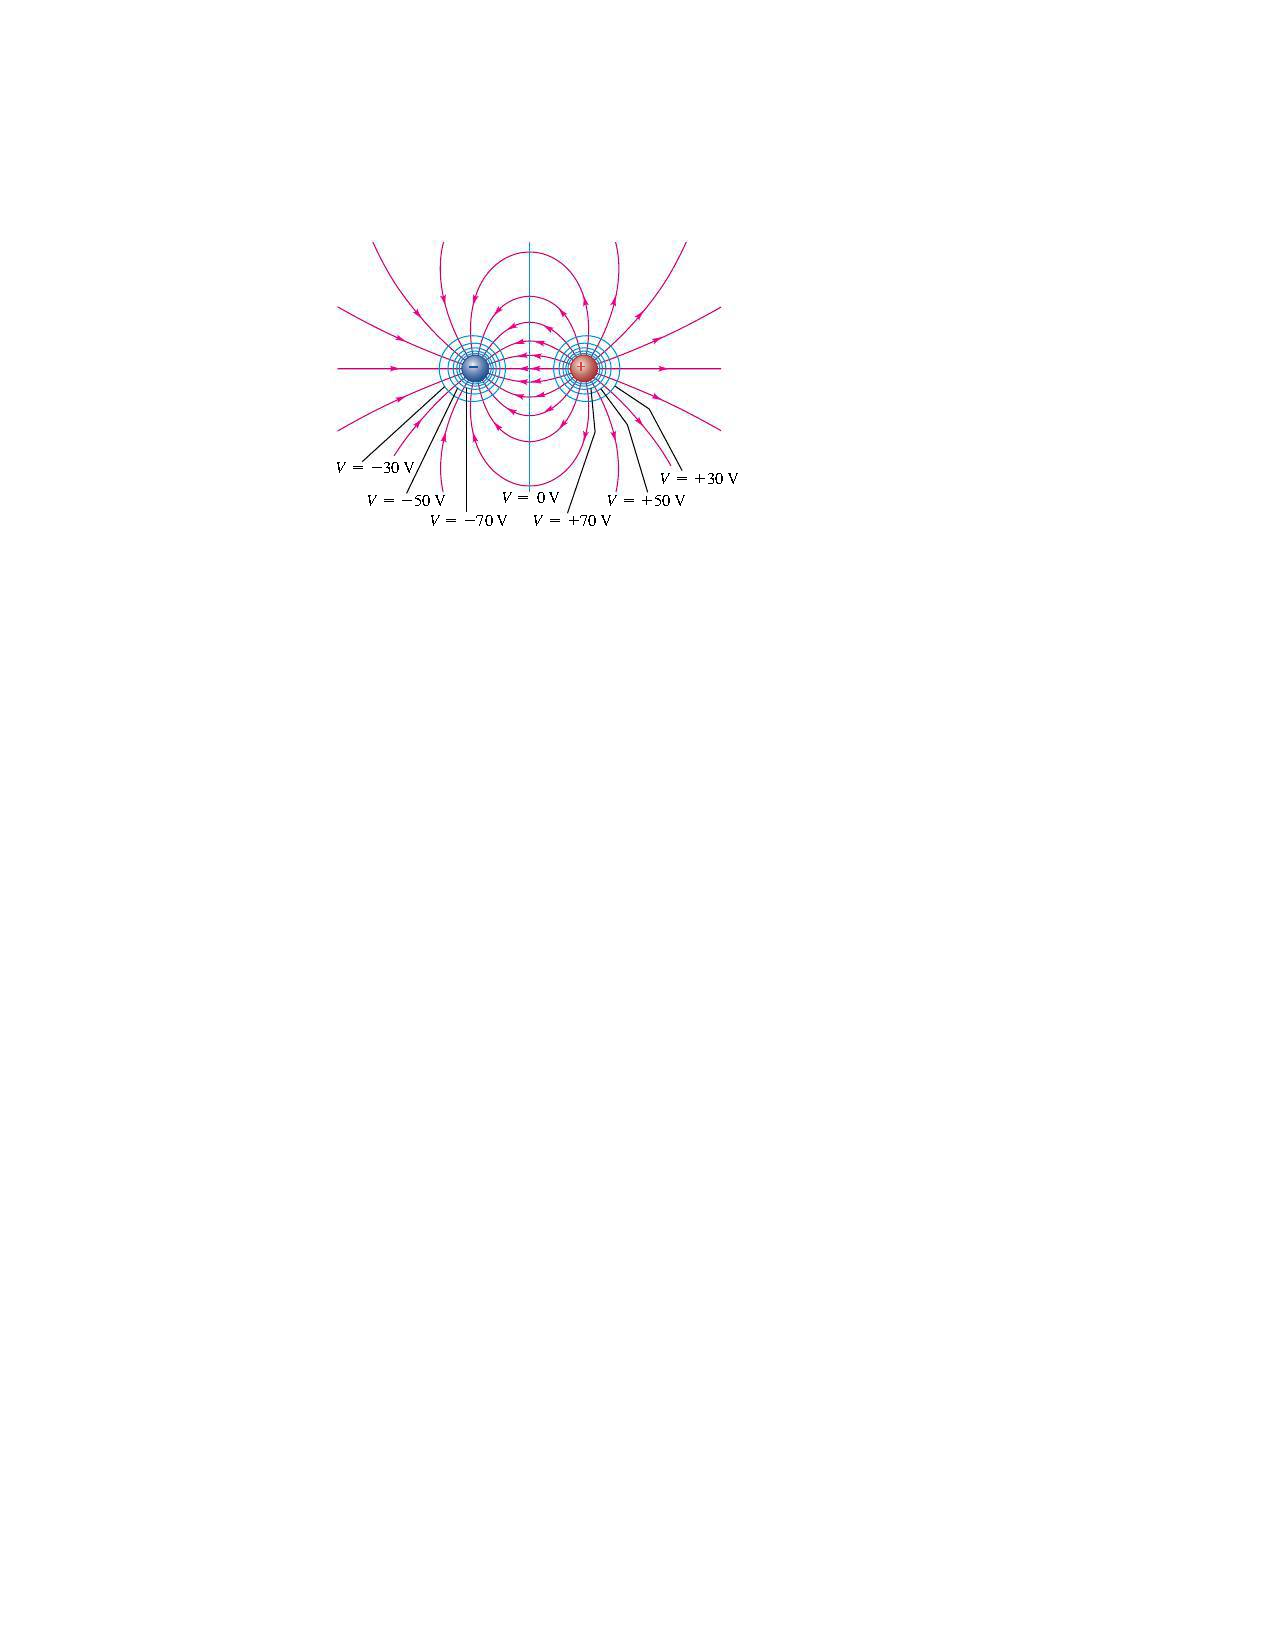
\includegraphics[center]{23-23b}
\center \textbf{Fig.~23.23b}
\end{minipage}

\vfill

\clearpage

\paragraph{Problem 23.81}
\begin{problem}
	A heart cell can be modeled as a cylindrical shell that is \SI{100}{\micro\meter} long, with an outer diameter of \SI{20.0}{\micro\meter} and a cell wall thickness of \SI{1.00}{\micro\meter}.  Potassium ions move across the cell wall, depositing positive charge on the outer surface and leaving a net negative charge on the inner surface.  During the so-called resting phase, the inside of the cell has a potential that is \SI{90.0}{\milli\volt} lower than the potential on the outer surface.
	\begin{enumerate}
		\item If the net charge of the cell is zero, what is the magnitude of the total charge on either cell wall membrane?  Ignore edge effects and treat the cell as a very long cylinder.
		\item What is the magnitude of the electric field just inside the cell wall?
		\item In a subsequent depolarization event, sodium ions move through channels in the cell wall, so that the inner membrane becomes positively charged.  At the end of this event, the inside of the cell has a potential that is \SI{20.0}{\milli\volt} higher than the potential outside the cell.  If we model this event by charge moving from the outer membrane to the inner membrane, what magnitude of charge moves across the cell wall during this event?
		\item If this were done entirely by the motion of sodium ions, Na$^+$, how many ions have moved?  
	\end{enumerate}
\end{problem}

\vfill

\end{document}